\section{Generative Adversarial Networks}
\label{sec:gan}

The networks so far learned a mapping from an image $x$ to a label $y$ that a
human supplied. A generative model reverses the direction of interest: it
should produce \emph{new} images that look as if they came from the training
set. No one can label what a ``correct'' new face or bedroom is, so the model
must learn from unlabeled images alone. A generative adversarial network (GAN)
solves this with a trick. A second network, the discriminator, tries to tell
generated images from real ones, and its mistakes and successes become the
training signal for the generator. This section first places GANs among
learning settings without labels, then derives the adversarial loss, explains
why GAN training is difficult and how the Wasserstein loss helps, and finally
shows conditional GANs and image translation models such as Pix2Pix, CycleGAN,
and StyleGAN.

\subsection{Learning Without Human Labels}

Learning settings differ in where the targets come from. In \emph{supervised
learning}, each training input $x$ comes with a human-provided label $y$, and
classification is the standard task. The CNNs, ResNets, and transformer
classifiers of the previous sections are supervised. In \emph{unsupervised
learning}, the data have no labels; clustering, density estimation, and
generative modeling are typical tasks, as in the density estimates of
Section~\ref{sec:bayes}. \emph{Self-supervised learning} lies in between:
it uses a supervised loss, but its labels are generated automatically from the
data or from the way the data were acquired. No annotator is needed, so large
unlabeled collections become usable.

Several acquisition setups deliver such labels for free. A video provides the
next frame a short time later, so predicting future frames has a known target.
A stereo camera provides a second view; predicting it from the first view can
be checked against the image the second camera actually recorded. A
high-frame-rate camera can generate sharp frames and, by averaging them,
realistic motion-blurred images, giving training pairs for recovering video
from motion blur. Even a segmentation can be checked without labels if one
assumes that a correct segmentation produces regions with typical low-level
features, while a wrong segmentation produces unusual ones.

Related settings relax the labels in other ways. \emph{Weakly supervised
learning} uses labels that are incomplete (only some examples labeled), inexact
(coarse, e.g. an image-level tag instead of a pixel mask), or inaccurate
(noisy). \emph{Domain adaptation} transfers a model to data with a different
appearance, and \emph{continual learning} keeps learning new tasks without
forgetting earlier ones. \emph{Pretext task learning} solves an artificial task
only as preparation for the actual \emph{downstream task}: the network trained
on the pretext task provides features, and a small labeled dataset suffices
for the downstream classifier.

\paragraph{Pretext tasks.}
Table~\ref{tab:pretext} lists common pretext tasks for images. The first four
remove or damage information and train an encoder--decoder network to restore
it. An autoencoder must squeeze the image through a narrow coarse feature layer
and reconstruct it; a denoising autoencoder additionally applies a distortion
$d(I)$, such as noise, before the encoder. Inpainting predicts a hidden image
region from its surroundings, and colorization predicts color from a grayscale
image. The last two are \emph{classification} tasks. For a jigsaw puzzle, the
image is cut into $n$ tiles and shuffled, and the network predicts which of the
$n!$ permutations was applied (in practice a subset of them). For context
prediction, the network sees two patches and predicts their discrete spatial
relation, e.g. ``top right.'' Self-supervised objectives are therefore not
necessarily regression tasks: whether the target is a pixel value or a class
index depends on how the pretext task is phrased. After pretraining, only the
encoder is kept and reused for the downstream task.

\begin{table}[ht]
  \centering
  \begin{tabular}{@{}p{3.3cm}p{4.0cm}p{3.8cm}p{2.9cm}@{}}
    \toprule
    Pretext task & Input & Target & Loss type \\
    \midrule
    Autoencoding & image & same image & regression \\
    Denoising & distorted image $d(I)$ & clean image $I$ & regression \\
    Inpainting & image with hidden region & hidden region & regression \\
    Colorization & grayscale image & color channels & regression or
      classification \\
    Jigsaw puzzle & shuffled tiles & index of permutation & classification \\
    Context prediction & two patches & relative position & classification \\
    Frame order & shuffled video frames & correct order & classification \\
    \bottomrule
  \end{tabular}
  \caption{Pretext tasks create targets from unlabeled data. Some predict
  pixels (regression); others predict a discrete arrangement
  (classification).}
  \label{tab:pretext}
\end{table}

\noindent
Two further self-supervised families, contrastive learning and energy-based
self-supervision, compare views of images instead of reconstructing them; they
are summarized in Appendix~\ref{app:ssl}.

\subsection{Latent Variables and Generative Models}

Most unsupervised models relate a data example $x$ to an unobserved
\emph{latent variable} $z$. Usually $z$ is much smaller than $x$ and can be
seen as a compressed description of it. Some models map from data to latent
space: $k$-means maps $x$ to a cluster index $z$, and the encoder of an
autoencoder maps an image to an embedding vector $z$. Other models map from
latent space to data space. If $z$ has a simple distribution $Pr(z)$, for
example a standard normal distribution, one can draw $z$ and map it to a new
example $x$. Models of this kind are called \emph{generative models}.
Figure~\ref{fig:gen-taxonomy} shows how these groups overlap.

\begin{figure}[ht]
  \centering
  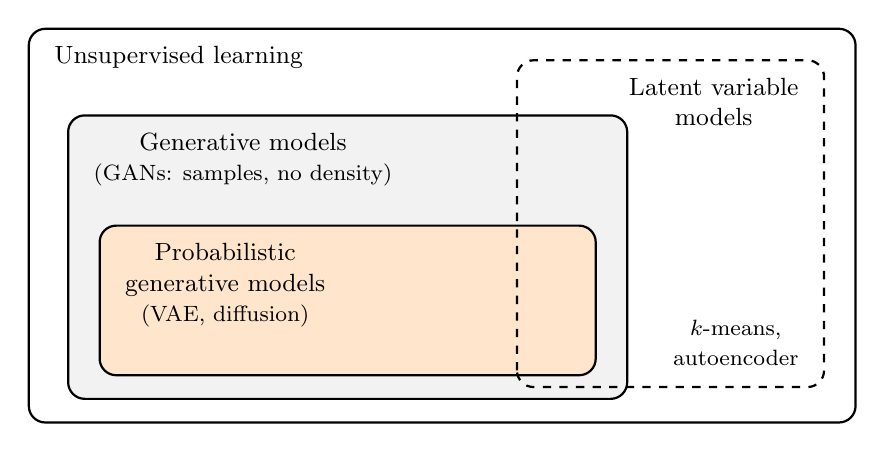
\begin{tikzpicture}[
    region/.style={draw, rounded corners=6pt, thick, align=left},
    lbl/.style={font=\small, align=center}
  ]
    \draw[region] (0,0) rectangle (10.5,5.0);
    \node[lbl, anchor=north west] at (0.2,4.9) {Unsupervised learning};
    \draw[region, fill=gray!10] (0.5,0.3) rectangle (7.6,3.9);
    \node[lbl, anchor=north west] at (0.7,3.8) {Generative models\\
      \footnotesize (GANs: samples, no density)};
    \draw[region, fill=orange!20] (0.9,0.6) rectangle (7.2,2.5);
    \node[lbl, anchor=north west] at (1.1,2.4) {Probabilistic\\ generative models\\
      \footnotesize (VAE, diffusion)};
    \draw[region, dashed] (6.2,0.45) rectangle (10.1,4.6);
    \node[lbl, anchor=north east] at (9.9,4.5) {Latent variable\\ models};
    \node[lbl, anchor=south east] at (9.9,0.6) {\footnotesize $k$-means,\\
      \footnotesize autoencoder};
  \end{tikzpicture}
  \caption{Taxonomy of unsupervised models. Generative models can create new
  examples; probabilistic generative models additionally assign a probability
  to every example. Latent variable models (dashed) cut across both groups.}
  \label{fig:gen-taxonomy}
\end{figure}

\noindent
A \emph{probabilistic} generative model, such as a variational autoencoder
(VAE) or a diffusion model, defines a probability $Pr(x_i\mid\phi)$ for every
data point given its parameters $\phi$. Training maximizes the probability of
the observed data, i.e. it minimizes the negative log-likelihood
\begin{equation}
  L[\phi] = -\sum_{i=1}^{I}\log Pr(x_i\mid\phi),
  \label{eq:gen-nll}
\end{equation}
\noindent
exactly as in maximum likelihood estimation (Equation~\ref{eq:ml}). As training
proceeds, the density rises where the training examples lie. A VAE thereby
learns an approximation of the data distribution. A GAN is different. It is
\emph{not} probabilistic: it provides a mechanism that turns random $z$ into
samples, but it cannot say how probable a given image is. Whether a method
\emph{estimates a distribution over the data} thus separates the methods in
Table~\ref{tab:density-vs-sampler}. Parzen windows and maximum likelihood fit a
density; a (restricted) Boltzmann machine defines one through an energy,
$p(x)\propto\exp(-E(x))$; a GAN does not.

\begin{table}[ht]
  \centering
  \begin{tabular}{@{}p{4.0cm}p{3.6cm}p{6.4cm}@{}}
    \toprule
    Method & Explicit density? & What it provides \\
    \midrule
    Parzen windows & yes & $\hat p(x)$ as sum of windows around samples \\
    Maximum likelihood & yes & parameters of a chosen density model \\
    (Restricted) Boltzmann machine & yes (unnormalized) & energy $E(x)$,
      $p(x)\propto e^{-E(x)}$ \\
    VAE, diffusion model & yes (approximate) & likelihood bound and samples \\
    GAN & no & samples $x^*=g[z,\theta]$ only \\
    \bottomrule
  \end{tabular}
  \caption{Density estimators versus samplers. A GAN generator produces
  examples whose distribution should match the data, but it never represents
  that distribution as a function that can be evaluated.}
  \label{tab:density-vs-sampler}
\end{table}

\paragraph{Measuring sample quality.}
Without a likelihood, a GAN must be judged by its samples. A pretrained
classifier gives a practical test with two parts. First, if a generated image
$x^*$ is realistic, the classifier should be confident: $Pr(y\mid x^*)$ should
be peaked at one class. Second, if the model generates all classes equally
often, the marginal class distribution averaged over $I$ samples,
\begin{equation}
  Pr(y) = \frac{1}{I}\sum_{i=1}^{I} Pr(y\mid x_i^*),
  \label{eq:gan-marginal}
\end{equation}
\noindent
should be flat. The \emph{inception score} combines both by measuring how far
each peaked $Pr(y\mid x_i^*)$ lies from the flat $Pr(y)$ with the KL divergence
of Equation~\ref{eq:kl}, averaged over samples: it is large only for images
that are both recognizable and varied. A generator that always draws the same
convincing dog passes the first test and fails the second.

\subsection{Adversarial Training}

A GAN consists of two networks. The \emph{generator} $g[z,\theta]$ maps a
latent vector $z$, drawn from a simple base distribution such as a standard
normal, to a sample $x^* = g[z,\theta]$ in image space. The
\emph{discriminator} $f[x,\phi]$ receives either a real training image $x_i$ or
a generated image $x_j^*$ and outputs the probability that its input is real.
If the discriminator cannot distinguish the two, the generator produces
plausible samples. If it can, the way it distinguishes them tells the generator
how to improve. Figure~\ref{fig:gan-pipeline} shows the arrangement.

\begin{figure}[ht]
  \centering
  \begin{tikzpicture}[
    box/.style={draw, rounded corners=2pt, minimum width=2.0cm,
      minimum height=0.9cm, align=center, font=\small},
    link/.style={-{Latex[length=2mm]}, thick},
    lbl/.style={font=\footnotesize, align=center}
  ]
    \node (z) at (0,0) {$z_j\sim\mathcal N(0,I)$};
    \node[box, fill=orange!25] (g) at (2.9,0) {Generator\\$g[z,\theta]$};
    \node (xs) at (5.4,0) {$x_j^*$};
    \node (xr) at (5.4,1.5) {$x_i$};
    \node[box, fill=gray!15] (d) at (8.2,0.75) {Discriminator\\
      $\mathrm{sig}[f[x,\phi]]$};
    \node[lbl] (out) at (11.4,0.75) {$Pr(\text{real})$};
    \draw[link] (z) -- (g);
    \draw[link] (g) -- (xs);
    \draw[link] (xs) -- (d.west |- 0,0.45);
    \draw[link] (xr) -- (d.west |- 0,1.05);
    \draw[link] (d) -- (out);
    \node[lbl, above=0.05cm of xr] {real examples};
    \node[lbl, below=0.05cm of xs] {generated samples};
    \draw[-{Latex[length=2mm]}, dashed] (out.south) -- ++(0,-1.9) -|
      node[lbl, pos=0.25, below] {gradient passes back through the
      discriminator into $\theta$} (g.south);
  \end{tikzpicture}
  \caption{GAN training. The discriminator sees real images $x_i$ and
  generated images $x_j^*$ and outputs the probability of ``real.'' Its output
  is differentiated with respect to the generator parameters $\theta$ by
  backpropagating through the discriminator (dashed path).}
  \label{fig:gan-pipeline}
\end{figure}

\paragraph{A one-dimensional example.}
Let the real data be scalars clustered around some value, and let the
generator merely shift standard normal noise, $x_j^* = g[z_j,\theta] = z_j +
\theta$. The single parameter $\theta$ moves all generated samples along the
axis. Suppose $\theta=3$ while the real samples lie around $7$. A
discriminator in the form of a logistic curve over $x$ easily separates the
two groups: $Pr(\text{real})$ is near $0$ for the synthesized samples and near
$1$ for the real ones. The generator improves by increasing $\theta$, because
that moves its samples up the logistic curve. At $\theta=4.9$ the groups
overlap partly; at $\theta\approx7$ they coincide and the best the
discriminator can do is a nearly flat curve. Training is a race in which each
network keeps adapting to the other.

\paragraph{The discriminator as a binary classifier.}
The discriminator solves a two-class problem with label $y=1$ for real and
$y=0$ for generated. A Bernoulli distribution with parameter
$\lambda\in[0,1]$ models such a label:
\begin{equation}
  Pr(y\mid\lambda) = (1-\lambda)^{1-y}\,\lambda^{y}.
  \label{eq:bernoulli}
\end{equation}
\noindent
The network output $f[x,\phi]$ is an arbitrary real number, so the logistic
sigmoid $\mathrm{sig}[a]=1/(1+e^{-a})$ maps it into $[0,1]$ and gives
$\lambda=\mathrm{sig}[f[x,\phi]]$. The negative log-likelihood of $I$ labeled
examples is the \emph{binary cross-entropy}
\begin{equation}
  L[\phi] = \sum_{i=1}^{I}
    -(1-y_i)\log\bigl(1-\mathrm{sig}[f[x_i,\phi]]\bigr)
    - y_i\log\mathrm{sig}[f[x_i,\phi]].
  \label{eq:bce}
\end{equation}

\paragraph{Why cross-entropy measures a distance.}
The name ``cross-entropy'' comes from comparing two distributions. The
Kullback--Leibler divergence between the empirical distribution $q$ of the
observed labels and the model distribution $Pr(y\mid\theta)$ is
\begin{equation}
  D_{KL}\bigl[q\,\|\,p\bigr] = \int q(y)\log q(y)\,dy
    - \int q(y)\log Pr(y\mid\theta)\,dy .
  \label{eq:kl}
\end{equation}
\noindent
The first term does not depend on $\theta$. Placing the empirical distribution
at the observed data, $q(y)=\frac1I\sum_i\delta[y-y_i]$, turns the second
term into $-\frac1I\sum_i\log Pr(y_i\mid\theta)$. Minimizing the KL divergence
therefore equals minimizing the negative log-likelihood, and with a Bernoulli
model this is exactly Equation~\ref{eq:bce}. The GAN loss can thus be read as a
distance between probability distributions.

\paragraph{The GAN loss.}
Insert $y=1$ for the real examples $x_i$ and $y=0$ for the generated samples
$x_j^*$. The discriminator minimizes
\begin{equation}
  L[\phi] = \sum_j -\log\bigl(1-\mathrm{sig}[f[x_j^*,\phi]]\bigr)
            - \sum_i \log\mathrm{sig}[f[x_i,\phi]] .
  \label{eq:gan-disc}
\end{equation}
\noindent
The generator wants its samples to be misclassified, so it \emph{maximizes} the
same loss with respect to $\theta$, after substituting $x_j^* =
g[z_j,\theta]$:
\begin{equation}
  \hat\theta = \operatorname*{argmax}_{\theta}\Bigl[\min_{\phi}\Bigl[
    \sum_j -\log\bigl(1-\mathrm{sig}[f[g[z_j,\theta],\phi]]\bigr)
    - \sum_i \log\mathrm{sig}[f[x_i,\phi]]\Bigr]\Bigr].
  \label{eq:gan-minimax}
\end{equation}
\noindent
This is a \emph{minimax game}: the discriminator parameters minimize the loss,
the generator parameters maximize it. The real-data term does not depend on
$\theta$, so the generator's part reduces to minimizing
\begin{equation}
  L[\theta] = \sum_j \log\bigl(1-\mathrm{sig}[f[g[z_j,\theta],\phi]]\bigr).
  \label{eq:gan-gen}
\end{equation}
\noindent
Training alternates: a gradient step on $\phi$ with a minibatch of real and
generated images, then a gradient step on $\theta$ with new samples, keeping
the other network fixed each time. The gradient of $L[\theta]$ flows from the
discriminator output back through the discriminator's layers, into the image
$x^*$, and from there into the generator. Generator backpropagation therefore
\emph{depends on the discriminator}; the generator never sees a real image
directly and learns only through the discriminator's judgment. At the ideal
end point, the generator draws samples from the real data distribution and the
discriminator can only guess, outputting $0.5$ everywhere.

For a numerical check, let the discriminator output $0.9$ for a real image and
$0.2$ for a generated one. Their contributions to Equation~\ref{eq:gan-disc}
are $-\log 0.9\approx0.105$ and $-\log(1-0.2)\approx0.223$, so
$L[\phi]\approx0.33$. The generator's term is $\log(1-0.2)\approx-0.223$; it
decreases if the discriminator's output for the generated image rises toward
$1$. At the equilibrium with outputs of $0.5$, each example contributes
$\log 2\approx0.693$. In practice the generator often minimizes
$-\log\mathrm{sig}[f[g[z,\theta],\phi]]$ instead of
Equation~\ref{eq:gan-gen}. Both push in the same direction, but the
alternative gives large gradients early in training, when the discriminator
confidently rejects all samples and $\log(1-\mathrm{sig}[\cdot])$ is almost
flat.

Two statements summarize what a GAN does and does not learn. It needs no
labeled pairs $(x,y)$: the labels real and generated are created by the
training procedure itself, so an unconditional GAN is unsupervised.
And although the distribution of its samples should approach the data
distribution, the generator never learns an explicit probability function of
the data; it learns a mapping from $z$ to images. Even when all generated
samples are indistinguishable from real ones, this does not guarantee that
every plausible image can be generated.

\subsection{DCGAN and Training Difficulties}

The deep convolutional GAN (DCGAN) uses convolutional networks for both roles
(Table~\ref{tab:dcgan}). The generator projects a $100$-dimensional latent
vector to a $4\times4\times1024$ tensor and reshapes it. Four fractionally
strided (transposed) convolutions each double the resolution and halve the
channels until a $64\times64\times3$ image emerges. A final $\tanh$ maps
pixel values to $[-1,1]$. The discriminator mirrors this path with strided
convolutions that halve the resolution, a final $4\times4$ convolution to a
single number, and a sigmoid. DCGANs produce convincing faces and bedroom
scenes, while samples trained on the diverse ImageNet classes remain
blurry object fragments.

\begin{table}[ht]
  \centering
  \begin{tabular}{@{}p{4.3cm}p{4.3cm}p{5.4cm}@{}}
    \toprule
    Generator stage & Output size & Operation \\
    \midrule
    latent $z$ & $100\times1$ & sampled from $\mathcal N(0,I)$ \\
    project and reshape & $4\times4\times1024$ & linear layer \\
    upsampling $1$--$3$ & $8\times8\times512$ to $32\times32\times128$ &
      fractionally strided conv. \\
    output & $64\times64\times3$ & fractionally strided conv., $\tanh$ \\
    \midrule
    Discriminator stage & Output size & Operation \\
    \midrule
    input $x$ or $x^*$ & $64\times64\times3$ & \\
    downsampling & $32\times32\times128$ to $4\times4\times1024$ & strided
      conv. \\
    output & $1\times1$ & $4\times4$ conv., sigmoid \\
    \bottomrule
  \end{tabular}
  \caption{DCGAN architecture. The generator doubles the resolution and halves
  the channels at each stage; the discriminator mirrors it.}
  \label{tab:dcgan}
\end{table}

\noindent
The latent space of a trained DCGAN has meaningful directions. Averaging the
latent vectors of several ``man with glasses'' images, subtracting the average
for ``man without glasses,'' and adding that for ``woman without glasses''
yields vectors that generate women with glasses. The discriminator's features
are also useful for image classification.

\paragraph{Why GANs are hard to train.}
DCGAN needed special measures to train at all: strided convolutions instead of
pooling for down- and upsampling, batch normalization in both networks, leaky
ReLU activations, and the Adam optimizer. An MLP generator with a similar
number of parameters and layers produced repetitive, low-quality bedrooms.
Two failure patterns are typical. In \emph{mode dropping}, the samples cover
only a subset of the data, for example only some face types. In \emph{mode
collapse}, the generator ignores its latent input and maps every $z$ to nearly
the same output. Both are rewarded by the discriminator as long as the few
produced images are realistic, because the loss of Equation~\ref{eq:gan-gen}
judges each sample separately.

An analysis of the loss as a distance between distributions shows two effects.
Regions with generated samples but no real examples are penalized, so the loss
enforces \emph{quality}. Regions with real examples but no samples are also
penalized, so it enforces \emph{coverage}. The problem lies in the gradient.
If generated and real distributions do not overlap, as for $\theta=3$ in the
one-dimensional example, an optimal discriminator is almost exactly $0$ on one
group and $1$ on the other. Its output is then flat around the samples, and
small changes of the generator distribution toward the real one hardly change
the loss. The generator receives little guidance about which way to move.

\subsection{Wasserstein GANs}

A better loss should decrease smoothly as the generated distribution moves
toward the real one, even when the two do not overlap. The \emph{Wasserstein
distance}, also called the \emph{earth mover's distance}, has this property. It
views each distribution as a pile of earth and measures the minimal cost of
reshaping the first pile into the second, where moving a unit of mass costs the
distance it travels. For discrete distributions $Pr(x=i)$ and $q(x=j)$, the
mass moved from bin $i$ to bin $j$ is stored in a \emph{transport plan} matrix
$P$:
\begin{equation}
  D_w\bigl[Pr(x)\,\|\,q(x)\bigr] = \min_{P}\sum_{i,j} P_{ij}\,|i-j|
  \quad\text{s.t.}\quad
  \sum_j P_{ij}=Pr(x=i),\;\;
  \sum_i P_{ij}=q(x=j),\;\;
  P_{ij}\ge0 .
  \label{eq:wasserstein-discrete}
\end{equation}
\noindent
The row sums use up the initial distribution, the column sums build the target
distribution, and masses cannot be negative. The objective and all constraints
are linear in $P$, so computing $D_w$ is a \emph{linear programming} problem.

For a worked example, take three bins with $Pr=(0.5,0.5,0)$ and
$q=(0,0.5,0.5)$. One optimal plan moves $0.5$ from bin $1$ to bin $2$ and $0.5$
from bin $2$ to bin $3$, with cost $0.5\cdot1+0.5\cdot1=1$. Moving $0.5$
directly from bin $1$ to bin $3$ costs $0.5\cdot2=1$ as well. In one dimension,
the result equals the summed absolute difference of the cumulative
distributions, $|0.5-0|+|1-0.5|+|1-1|=1$. Shifting $q$ one bin further right
raises the distance to $2$. The KL divergence, in contrast, is infinite for
both shifted versions because $q$ puts mass where $Pr$ has none; it cannot tell
``close'' from ``far.''

For continuous distributions, the plan becomes a joint density
$\pi(x_1,x_2)$ describing the mass moved from $x_1$ to $x_2$:
\begin{align}
  D_w\bigl[Pr(x),q(x)\bigr]
  &= \min_{\pi}\iint \pi(x_1,x_2)\,\|x_1-x_2\|\,dx_1\,dx_2 \notag\\
  &= \max_{f:\;|\partial f/\partial x|\le1}
    \Bigl[\int Pr(x)f[x]\,dx - \int q(x)f[x]\,dx\Bigr].
  \label{eq:wasserstein-dual}
\end{align}
\noindent
The right-hand form is the dual linear program. It searches over functions
$f[x]$ whose slope is at most $1$ (\emph{1-Lipschitz}) for the one that best
separates the two distributions by their average values. A neural network
$f[x,\phi]$ can approximate this function. Replacing the integrals with
averages over samples gives the \emph{Wasserstein GAN} (WGAN) loss for the
network, often called the critic:
\begin{equation}
  L[\phi] = \sum_j f[x_j^*,\phi] - \sum_i f[x_i,\phi]
          = \sum_j f[g[z_j,\theta],\phi] - \sum_i f[x_i,\phi],
  \qquad \Bigl|\frac{\partial f[x,\phi]}{\partial x}\Bigr| < 1 .
  \label{eq:wgan}
\end{equation}
\noindent
The critic is minimized with respect to $\phi$ and the generator maximizes it,
as before. Three differences from the cross-entropy GAN matter. The critic has
\emph{no sigmoid}: its output is a scalar score, not a probability. The
Lipschitz constraint bounds its slope to at most $45^\circ$, so it cannot
become an infinitely steep step between the groups. And because of this bounded
slope, the critic keeps a useful gradient even when the two distributions are
far apart. In the one-dimensional example, $D_w$ equals the distance between
the two clusters, $|7-\theta|$, and its gradient with respect to $\theta$ never
vanishes.

In practice, the Wasserstein loss always provides meaningful gradients, reduces
the likelihood of mode collapse, and correlates with the visual quality of the
samples, so it can be used to monitor training. It does not solve everything.
The ground distance $\|x_1-x_2\|$ is measured between pixel vectors, and
Euclidean pixel distance differs from human perceptual similarity. WGAN losses
therefore do not perfectly track visual quality, and training still requires
care.

\subsection{Improving Quality and Diversity}

Several further techniques, often combined, allow GANs to synthesize varied,
realistic images at high resolution.
Table~\ref{tab:gan-improvements} summarizes their purpose.

\begin{table}[ht]
  \centering
  \begin{tabular}{@{}p{4.0cm}p{5.0cm}p{5.0cm}@{}}
    \toprule
    Technique & Change & Main effect \\
    \midrule
    Wasserstein loss & critic without sigmoid, 1-Lipschitz & useful gradients,
      less mode collapse \\
    Progressive growing & add layers for higher resolution & stable
      high-resolution training \\
    Minibatch discrimination & batch statistics in discriminator & diversity \\
    Truncation $\tau$ & reject far-out latent values & quality at the cost of
      diversity \\
    Precision / recall & compare real and synthetic manifolds & measure
      quality and coverage separately \\
    \bottomrule
  \end{tabular}
  \caption{Improvements to GAN training and evaluation. Most trade off or
  separately control sample quality and diversity.}
  \label{tab:gan-improvements}
\end{table}

\paragraph{Progressive growing.}
Training starts with a generator and discriminator for $4\times4$ images.
Once they are stable, both receive additional layers for the next resolution,
$8\times8$, and so on up to $1024\times1024$. The new higher-resolution layers
\emph{fade in} over several iterations, mixed with an upsampled version of the
previous output, so they do not disturb what the lower layers already learned.
Coarse structure is thus settled before fine detail is learned.

\paragraph{Minibatch discrimination.}
Mode collapse goes unnoticed if the discriminator judges images one at a time.
With minibatch discrimination, the discriminator also computes feature
statistics across the whole minibatch, separately for real and synthesized
data, and uses them in its decision. A batch of near-identical samples then
looks unlike a batch of real images, and the generator is pushed to produce
the same variety as the real data.

\paragraph{Truncation.}
Samples from the tails of the latent distribution tend to be less realistic.
Rejecting latent values that fall further than $\tau$ standard deviations from
the mean trades diversity for quality. With $\tau=2$, generated dogs vary
strongly in pose and background; with $\tau=0.04$, they all look nearly the
same, but each is very clean.

\paragraph{Manifold precision and recall.}
Quality and diversity can be measured separately. Approximate the real
manifold by the union of small spheres around real examples, and the synthetic
manifold likewise around generated samples, usually in a feature space rather
than in pixel space. \emph{Precision} is the fraction of generated samples that
fall inside the real manifold and measures quality. \emph{Recall} is the
fraction of real examples that fall inside the synthetic manifold and measures
coverage. Truncation raises precision and lowers recall.

\paragraph{Latent interpolation.}
Moving smoothly along a straight line between two latent vectors produces
realistic intermediate images, e.g. one car gradually turning into another.
Smooth interpolation shows that the generator has learned a continuous
representation rather than memorizing the individual training images.

\subsection{Conditional Generation}

The GANs discussed so far cannot be asked for an image of a specified kind; a
random $z$ yields a random class. Three variants add an attribute $c$, for
example a class, to control the output. Table~\ref{tab:gan-conditional}
compares them.

A \emph{conditional GAN} passes $c$ to both networks, $g[z,c,\theta]$ and
$f[x,c,\phi]$. For the generator, $c$ is simply appended to $z$. For the
discriminator, $c$ is first linearly transformed to a 2D map and added as an
extra channel of the input image. The discriminator then judges whether the
\emph{pair} $(x,c)$ is real. A generator that ignores $c$ is caught, because a
realistic cat paired with the label ``dog'' is not a real pair.

The \emph{auxiliary classifier GAN} (ACGAN) keeps the discriminator input
image-only but requires it to predict the attribute. For a discrete attribute
with $C$ categories, the discriminator has $C+1$ outputs: one sigmoid output
for real versus generated and a softmax over $C$ classes. The generator is
trained so that its samples are both judged real and classified as the class it
was asked for. ACGANs trained on ImageNet synthesize recognizable examples of
many classes, such as butterflies, birds, and flowers.

\emph{InfoGAN} tries to discover attributes automatically, without labels. The
generator takes random noise $z$ together with a random attribute vector $c$,
whose components may be discrete, like a class, or continuous. Besides the
real/generated output, the discriminator has a second head that estimates $c$
from the generated image. To make this estimate possible, the generator must
make $c$ visible in its output, and $c$ becomes a meaningful factor of
variation. On handwritten digits, a discrete $c$ with ten values ends up
selecting the digit, and continuous components control stroke slant and
thickness, even though no labels were used.

\begin{table}[ht]
  \centering
  \begin{tabular}{@{}p{2.6cm}p{3.2cm}p{4.0cm}p{4.2cm}@{}}
    \toprule
    Model & Attribute $c$ & Discriminator input & Discriminator output \\
    \midrule
    Conditional GAN & given (labels) & image and $c$ & pair is real \\
    ACGAN & given class & image & real, and class softmax ($C+1$) \\
    InfoGAN & random, no labels & image & real, and estimate of $c$ \\
    \bottomrule
  \end{tabular}
  \caption{Three ways to condition a GAN. They differ in whether the attribute
  is labeled and in how the discriminator checks it.}
  \label{tab:gan-conditional}
\end{table}

\subsection{Image Translation}

The adversarial discriminator was introduced to generate random samples, but it
also serves as a learned prior that favors \emph{realism} when one image is
translated into another. The generator then receives an image $c$ instead of,
or in addition to, noise, and produces an output image. A content loss keeps
the output related to its input or to a target, and an adversarial loss makes it
look real.

\paragraph{Pix2Pix.}
Pix2Pix maps an image $c$ to an image $x$ of a different style with a U-Net
$g[c,\theta]$ (Section~\ref{sec:resnet}). Examples are colorization, map to
aerial photo, sketch to product photo, and facade label map to facade photo.
Training requires \emph{paired} examples: for each input, the true output
image is known. Two losses combine. The content loss $\|x-g[c,\theta]\|_1$
compares the prediction with the ground truth. The $\ell_1$ norm alone gives
blurry results, because averaging several plausible outputs minimizes it. The
adversarial discriminator $f[c,x,\phi]$ therefore receives the before image and
an after image and learns to distinguish real before/after pairs from
before/synthesized pairs; its feedback trains the generator as usual. The input
$c$ plays the role of the condition in a conditional GAN.

\paragraph{Transcoding radar to optical images.}
Image translation also produces features for downstream tasks. Radar
satellites such as Sentinel-1 see through clouds, but their speckled images are
hard to interpret; optical Sentinel-2 images are easy to read but often cloudy.
A GAN trained on co-registered pairs \emph{transcodes} radar tiles into
synthetic optical tiles; the optical images are needed only for training. The
generator's learned radar features are then reused for land-cover
classification. With only a few hand-labeled samples, a classifier built on
these pretrained features, retraining only its last layers, reached about
$0.85$ accuracy even with $1/16$ of the labeled data. Random forests and CNNs
trained from scratch reached only about $0.4$ to $0.7$, and their accuracy
dropped as labeled data decreased. The GAN acts here as a pretext task in the
sense of the first subsection.

\paragraph{Super-resolution GAN.}
SRGAN upsamples a low-resolution image by a factor of four. The content loss
compares the prediction with the true high-resolution image, often in the
feature space of a pretrained VGG network rather than per pixel. The
discriminator differs from Pix2Pix: it does not judge before/after pairs, but
distinguishes the synthesized image from \emph{other} real high-resolution
images. The adversarial loss thus penalizes any output that looks synthetic.
Compared with bicubic upsampling, SRGAN produces sharp textures such as
individual branches and fabric patterns instead of blur.

\paragraph{CycleGAN.}
Often two image sets with distinct styles exist, but no matching pairs: photos
and Monet paintings, or horses and zebras. Pix2Pix cannot be trained without
pairs. CycleGAN relies on a consistency idea: translating a photo into a
painting and then back into a photo should recover the original.
It trains \emph{two generators}, $g$ from domain $A$ to $B$ and $g'$ from $B$
to $A$, and \emph{two discriminators}, one per domain, all simultaneously
(Figure~\ref{fig:cyclegan}). For an input $c$ from domain $A$, its loss is a
weighted sum of three terms. A content loss encourages the translated image
$g[c]$ to agree with $c$, so the scene is preserved. An adversarial loss
encourages $g[c]$ to be indistinguishable from real images of domain $B$. The
cycle-consistency loss $\|g'[g[c]]-c\|_1$ encourages the mapping to be
reversible. The same three terms are applied in the other direction, so there
are two content losses and two adversarial losses.

\begin{figure}[ht]
  \centering
  \begin{tikzpicture}[
    box/.style={draw, rounded corners=2pt, minimum width=1.9cm,
      minimum height=0.85cm, align=center, font=\small},
    img/.style={draw, minimum width=1.5cm, minimum height=0.85cm,
      align=center, font=\small},
    link/.style={-{Latex[length=2mm]}, thick},
    lbl/.style={font=\footnotesize, align=center}
  ]
    \node[img] (c) at (0,0) {horse $c$};
    \node[box, fill=orange!25] (g) at (3.0,0) {$g[c,\theta]$};
    \node[img] (cp) at (6.0,0) {zebra $c'$};
    \node[box, fill=orange!25] (gp) at (3.0,-2.0) {$g'[c',\theta']$};
    \node[img] (cr) at (0,-2.0) {horse $\hat c$};
    \node[box, fill=gray!15] (d) at (9.9,0) {Discriminator $B$};
    \node[img] (zr) at (6.0,1.6) {real zebra};
    \draw[link] (c) -- (g);
    \draw[link] (g) -- (cp);
    \draw[link] (cp.south) |- (gp.east);
    \draw[link] (gp) -- (cr);
    \draw[link] (cp) -- (d);
    \draw[link] (zr.east) -| (d.north);
    \draw[dashed, {Latex[length=2mm]}-{Latex[length=2mm]}] (c.south) --
      node[lbl, right] {cycle loss} (cr.north);
    \node[lbl, below=0.1cm of d] {adversarial loss:\\$c'$ looks real};
    \node[lbl, above=0.1cm of g] {content loss:\\$c'$ agrees with $c$};
  \end{tikzpicture}
  \caption{CycleGAN, direction horse to zebra. The generator $g$ translates, a
  discriminator judges realism in the zebra domain, and the second generator
  $g'$ maps back so that the cycle loss can compare $\hat c$ with $c$. The
  reverse direction adds a second discriminator for horses.}
  \label{fig:cyclegan}
\end{figure}

\paragraph{StyleGAN.}
A usual GAN feeds the latent variable only at the input of the generator.
StyleGAN instead injects latent information at \emph{various points} of the
architecture and separates two kinds of variation. The \emph{style} carries
variation salient to humans. A fully connected mapping network first turns the
latent $z$ into an intermediate variable $w$ of size $512$. At each scale, a
learned linear transform turns $w$ into a style vector $y_k$ of $2\times512$
values: a per-channel scale and offset. These are applied after normalizing
each channel of the feature map, as in instance normalization
(Table~\ref{tab:norm-variants}); the combination is called \emph{adaptive
instance normalization}. \emph{Noise} represents unimportant variation: at
each scale, fresh random noise maps, multiplied by learned per-channel factors,
are added to every channel. For faces, styles at coarse scales control face
shape and head pose, styles at medium scales the shape and details of facial
features, and styles at fine scales hair and skin color. Changing the noise
leaves the identity unchanged and only varies small details such as the exact
placement of hair strands and skin pores.

\paragraph{What the translation models need.}
Table~\ref{tab:gan-translation} compares the translation models. Only
Pix2Pix and SRGAN require paired ground truth; CycleGAN learns from unpaired
image sets, and unconditional GANs need no labels at all. Thus not all GANs
require labeled tuples $(x,y)$.

\begin{table}[ht]
  \centering
  \begin{tabular}{@{}p{2.2cm}p{2.9cm}p{4.2cm}p{4.7cm}@{}}
    \toprule
    Model & Training data & Losses & Discriminator judges \\
    \midrule
    Pix2Pix & paired images & $\ell_1$ content, adversarial & before/after
      pair is real \\
    SRGAN & paired low/high res. & VGG content, adversarial & image looks like
      real high-resolution image \\
    CycleGAN & two unpaired sets & content, adversarial, cycle (each twice) &
      image looks like its domain (two discriminators) \\
    StyleGAN & unlabeled images & adversarial & image looks real \\
    \bottomrule
  \end{tabular}
  \caption{Image translation and style models. Paired data allow a direct
  content loss; unpaired data require cycle consistency.}
  \label{tab:gan-translation}
\end{table}
